\documentclass[10pt,a4paper]{article}
\usepackage{fontspec}
\usepackage[spanish,es-noshorthands]{babel}
\usepackage[margin=2.2cm]{geometry}
\usepackage{amsmath,amssymb,booktabs,graphicx,siunitx,xcolor,caption,array,microtype}
\usepackage{xurl}
\usepackage{adjustbox}
\usepackage[colorlinks,linkcolor=teal,citecolor=teal,urlcolor=teal,pdftitle={Viviendas y población expuestas al aluvión de San Carlos de Apoquindo},pdfauthor={Lester Wood},pdflang={es-CL}]{hyperref}
\usepackage[natbibapa]{apacite}
\renewcommand{\doiprefix}{https://doi.org/\ignorespaces}
\AtBeginDocument{\renewcommand{\BRetrievedFrom}{}}
\sisetup{output-decimal-marker={,},group-separator={.},group-minimum-digits=4,group-digits=integer}
\captionsetup{font=small,labelfont=bf}
\graphicspath{{figs/}}

\title{Viviendas y población expuestas al aluvión de San Carlos de Apoquindo\\(Las Condes, 8 de octubre de 2026): estimación a partir de la\\propagación simulada, datos censales y curvas de vulnerabilidad}
\author{Lester Wood\thanks{Estudio independiente; documento derivado de \citet{wood2026}. Contenido bajo licencia CC BY-NC-SA 4.0. Condiciones de uso: \url{https://aluvion.hirely.cl/terminos.html}.}}
\date{Versión preliminar del 11 de octubre de 2026 (ciudad completa; método corregido)}

\begin{document}
\maketitle

\begin{abstract}
\noindent\textbf{Alcance.} Subestudio independiente basado exclusivamente en datos públicos. Sus resultados son calculados bajo supuestos y requieren validación científica independiente. No evalúa obras reales ni atribuye responsabilidades. Esta versión reemplaza a la del 9 de octubre, que usaba la primera generación del modelo (1.103 edificios).\par\medskip
\noindent Se calculó la exposición de edificios, viviendas y población censal a la propagación simulada del aluvión de San Carlos de Apoquindo, y la pérdida relativa esperada en los edificios. Para ello se cruzaron las huellas de propagación del estudio principal, con los 42.018 edificios representados, con las huellas de edificios y las 1.210 unidades censales del Censo 2017. El método incorpora las correcciones de una revisión automatizada: unidades censales disueltas, ponderación areal exacta, distancia real a la huella, curvas usadas solo en su dominio y pérdida agregada en lugar de «edificios destruidos».

En la hipótesis seleccionada, el área con más de \SI{5}{cm} de barro simulado tiene a 8~m o menos 3.950 edificios. Las viviendas asignadas a ella son 2.221 por ponderación areal y 5.827 por asignación dasimétrica, con un rango de 1.900 a 6.551 en la sensibilidad. Senapred informó 2.361 viviendas afectadas en su balance preliminar y 2.056 en el posterior. Con las curvas de vulnerabilidad y el espesor máximo simulado como intensidad, entre 366 y 593 viviendas quedan asignadas a edificios con una pérdida esperada de al menos 0,2, varias veces las 75 con daño mayor del balance preliminar y las 96 destruidas o con daño mayor del posterior.

Dos limitaciones condicionan estas cifras. La propagación no superó la prueba con observaciones reservadas del estudio principal: deja sin barro partes importantes de la zona afectada oficial y se extiende fuera de ella. Además, con los edificios representados como bloques, el barro se concentra en las calles con espesores altos que las curvas traducen en daño, aunque no necesariamente entró a las viviendas. Por eso las cifras son órdenes de magnitud condicionados al modelo, no una estimación del daño ocurrido.
\end{abstract}

\section{Introducción y planteamiento del problema}
La reconstrucción numérica del aluvión del 8 de octubre de 2026 \citep{wood2026} estima por dónde corrió el barro y con qué espesor y velocidad. Para la respuesta y la recuperación, la pregunta operativa es otra: cuántas viviendas y personas pudieron quedar expuestas, con qué intensidad, y cuántas viviendas pudieron sufrir daño importante. Las cifras públicas son balances levantados en terreno \citep{senapred2026latribuna,cnn2026balance,latercera2026senapred}, sin una distribución espacial publicada por vivienda. El visor de emergencia oficial publica la zona afectada y 2.266 predios afectados \citep{bbnn2026visor}. Este trabajo propone una estimación reproducible a partir de datos públicos, cuantifica su sensibilidad a los supuestos y la compara descriptivamente con esas cifras.

\section{Marco teórico}
\paragraph{Amenaza, exposición y vulnerabilidad.} En la terminología de las Naciones Unidas \citep{undrr2016}, la \emph{exposición} es la situación de las personas, la infraestructura y los bienes ubicados en zonas propensas a una amenaza, y la \emph{vulnerabilidad} es la susceptibilidad de esos elementos a sufrir daño. El riesgo resulta de combinar la amenaza (aquí, la intensidad del flujo de barro), la exposición y la vulnerabilidad. Este trabajo cuantifica las dos últimas a partir de la amenaza simulada.
\paragraph{Asignación espacial de la población.} Los censos entregan la población por unidades administrativas ---aquí, manzanas---, no por edificio. La \emph{ponderación areal} reparte la población de cada unidad en proporción al área intersectada y supone una densidad uniforme dentro de ella. Los métodos \emph{dasimétricos} usan información auxiliar, como la cobertura del suelo o las huellas de edificios, para concentrar la población donde efectivamente se ubica; reducen el error de la ponderación areal cuando la unidad contiene áreas no habitadas \citep{eicher2001,mennis2003}.
\paragraph{Vulnerabilidad física a flujos de detritos.} Las curvas de vulnerabilidad relacionan una medida de intensidad del proceso con el grado de pérdida $V\in[0,1]$, es decir, el costo de reparación sobre el valor del edificio. Para flujos de detritos, la intensidad más usada es la altura del depósito junto al edificio. \citet{fuchs2007} ajustaron un polinomio de segundo grado con datos del evento del 16 de agosto de 1997 en Wartschenbach (Austria), para edificios de albañilería y hormigón:
\begin{equation}
V_F(h)=0{,}11\,h^2-0{,}02\,h,\qquad h<\SI{2,5}{m},\qquad R^2=0{,}86. \label{eq:fuchs}
\end{equation}
\citet{papathoma2012} propusieron una función de Weibull con 51 edificios dañados en el evento de 1987 en el Tirol del Sur (Italia):
\begin{equation}
V_P(h)=1-\exp\!\left[-0{,}270\left(\frac{h+1{,}287}{1{,}287}-1\right)^{2{,}974}\right],\qquad R^2=0{,}835. \label{eq:pk}
\end{equation}
Ambas curvas son pequeñas para espesores bajo \SI{0,5}{m} y crecen con rapidez sobre \SI{1}{m}, cuando el barro supera las aberturas y entra a los edificios.

\section{Preguntas y objetivos}
La versión anterior planteaba dos hipótesis de concordancia con los balances oficiales. Esas hipótesis se formularon conociendo los balances, y un factor dos elegido así no constituye una prueba. Por eso se reemplazan por dos preguntas exploratorias:
\begin{description}
\item[P1] ¿En qué orden de magnitud quedan las viviendas asignadas al área con barro simulado respecto de las viviendas afectadas informadas, y cuánto depende ese orden del método de asignación?
\item[P2] ¿En qué orden de magnitud quedan las viviendas con pérdida esperada de al menos 0,2 respecto de las informadas con daño mayor o destruidas, y qué supuestos explican la diferencia?
\end{description}
\noindent\textbf{Objetivos:}
\begin{enumerate}
\item contar los edificios expuestos por clase de espesor;
\item estimar las viviendas y la población expuestas con dos métodos de asignación;
\item estimar la pérdida relativa esperada con dos curvas de vulnerabilidad;
\item cuantificar la sensibilidad a los supuestos;
\item comparar descriptivamente con las cifras oficiales.
\end{enumerate}

\section{Metodología}
\subsection{Datos}
\begin{table}[htbp]\centering\small
\caption{Datos utilizados.}\label{tab:datos}
\begin{tabular}{p{.2\textwidth}p{.42\textwidth}p{.3\textwidth}}\toprule
Dato & Fuente & Uso\\\midrule
Propagación simulada & Espesor máximo por celda en siete escenarios del estudio principal \citep{wood2026}, seis con los 42.018 edificios representados & Intensidad $h$ junto a cada edificio\\
Huellas de edificios & Overture Maps \citep{overture2026}: 42.018 huellas (OSM, Microsoft y Google) & Exposición física y asignación dasimétrica\\
Censo 2017 & INE \citep{ine2017manzanas}: 1.221 registros que corresponden a 1.210 unidades censales, con 62.695 viviendas y 178.470 personas & Viviendas y personas por unidad\\
Cifras oficiales & Senapred y Municipalidad de Las Condes \citep{senapred2026latribuna,cnn2026balance,latercera2026senapred}; visor de emergencia \citep{bbnn2026visor} & Comparación descriptiva (no se usan para calibrar)\\
Herramienta & Procedimiento de análisis territorial de Hirely Broker \citep{hirelybroker2026} & Selección de fuentes y cruce territorial\\
\bottomrule\end{tabular}\end{table}

\paragraph{Declaración de interés.} Hirely Broker es un producto propio del autor. Sus datos se obtuvieron de la misma fuente pública que usa la herramienta. No se usó información de propietarios ni de roles prediales: el análisis es exclusivamente agregado.

\paragraph{Escenarios.} Se usan siete escenarios:
\begin{itemize}
\item la hipótesis seleccionada (z02: cauce principal, brazos sur y lluvia sobre la ladera, \SI{300000}{m^3});
\item la misma hipótesis con más rugosidad fuera de las calles (v27);
\item solo el cauce principal, con \SI{300000} y \SI{150000}{m^3} (v01 y v07);
\item dos escenarios hipotéticos con la capacidad del colector de Bulnes Correa fijada en 30 y \SI{100}{m^3/s} (v17 y v10), que no describen la obra real;
\item como referencia, el escenario seleccionado en la primera generación del modelo (e04).
\end{itemize}

\subsection{Unidades censales}
Algunas unidades censales vienen como varias geometrías con el mismo total de viviendas y personas, en particular las agrupaciones «901». Se disolvieron por su identificador, de modo que el total se cuenta una sola vez, y se recuperaron sus partes completas desde el servicio del INE. Esa consulta quedó en el registro probatorio. Nueve unidades quedan solo parcialmente dentro del dominio de las simulaciones; su parte exterior se trata como sin barro, lo que puede subestimar levemente su exposición.

\subsection{Intensidad junto a cada edificio}
Para cada edificio $b$ se toma como intensidad el espesor máximo simulado en las celdas a una distancia $r$ o menor de su huella:
\begin{equation}
h_b=\max_{\,i:\ d(\mathbf x_i,\,\text{huella}_b)\le r} h_{\max,i},
\end{equation}
con $r=\SI{8}{m}$ en el caso base, y 4 y \SI{16}{m} en la sensibilidad. El espesor máximo del flujo en la calle contigua es una cota superior del espesor del depósito junto al edificio, que es la intensidad que usan las curvas de vulnerabilidad.

\subsection{Viviendas y personas expuestas}
\paragraph{(A) Ponderación areal exacta.} La fracción $f_j(h^*)$ de cada unidad $j$ con espesor mayor al umbral se calcula sobre una retícula de \SI{4}{m}, con el espesor interpolado linealmente desde la malla:
\begin{equation}
V^{A}(h^*)=\sum_j f_j(h^*)\,V_j,\qquad P^{A}(h^*)=\sum_j f_j(h^*)\,P_j .
\end{equation}
\paragraph{(B) Asignación dasimétrica.} Las viviendas de cada unidad se reparten entre las huellas de 30 a \SI{2000}{m^2}, en proporción al área de la huella que cae dentro de la unidad:
\begin{equation}
v_b=\sum_j V_j\frac{|A_b\cap j|}{\sum_{b'}|A_{b'}\cap j|},\qquad V^{B}(h^*)=\sum_b v_b\,\mathbf 1[h_b>h^*],
\end{equation}
y análogamente para las personas. Las 18 unidades sin huellas elegibles (1.610 viviendas) se asignan por ponderación areal; esta alternativa queda declarada explícitamente.

\subsection{Pérdida relativa esperada}
Para cada edificio se evalúan $V_F(h_b)$ y $V_P(h_b)$ (ecuaciones~\ref{eq:fuchs} y~\ref{eq:pk}). La curva de Fuchs se usa solo en su dominio ($h<\SI{2,5}{m}$), recortada a cero donde el polinomio es negativo ($h<\SI{0,18}{m}$), y los edificios con $h\geq\SI{2,5}{m}$ se cuentan aparte. Se informan:
\begin{itemize}
\item la pérdida relativa agregada $\Sigma V$, que no es un conteo de edificios destruidos;
\item el número de edificios con $V\geq0{,}2$;
\item las viviendas asignadas a esos edificios.
\end{itemize}

\subsection{Sensibilidad y comparación}
La sensibilidad se evalúa variando el umbral ($h^*$ = 2, 5, 10 y \SI{30}{cm}), la distancia ($r$ = 4, 8 y \SI{16}{m}), el método (A o B) y el escenario. La comparación con las cifras oficiales es descriptiva. «Expuesta» significa dentro del área con barro simulado; «afectada» es la categoría administrativa del balance citado. No se presupone que ambas categorías sean equivalentes.

\subsection{Revisión de la metodología}
El método se sometió a una revisión automatizada con un segundo modelo de lenguaje (gpt-6-astra, Codex), documentada por el autor. No constituye una revisión científica independiente. Esta versión incorpora sus correcciones; el informe se publica junto al documento.

\section{Resultados}
\begin{table}[htbp]\centering\small
\caption{Exposición calculada por escenario con $h^*=\SI{5}{cm}$ y distancia a la huella $r=\SI{8}{m}$. (A) ponderación areal exacta por unidad censal; (B) asignación dasimétrica por área de huella. «$>$\SI{1}{m}»: edificios con más de \SI{1}{m} de espesor máximo simulado a \SI{8}{m} o menos.}\label{tab:exposicion}
\begin{adjustbox}{max width=\textwidth}\begin{tabular}{p{.36\textwidth}rrrrrr}\toprule
Escenario & Edificios & \multicolumn{2}{c}{Viviendas} & \multicolumn{2}{c}{Personas} & Edificios\\\cmidrule(lr){3-4}\cmidrule(lr){5-6}
 & $>$\SI{5}{cm} & (A) & (B) & (A) & (B) & $>$\SI{1}{m}\\\midrule
Seleccionada: cauce + brazos sur + lluvia (300 mil m³) & 3.950 & 2.221 & 5.827 & 7.052 & 17.883 & 599\\
Ídem con más rugosidad fuera de calles & 3.212 & 1.930 & 4.676 & 6.233 & 14.701 & 577\\
Solo cauce principal (300 mil m³) & 2.597 & 1.589 & 3.813 & 5.166 & 11.897 & 556\\
Solo cauce principal (150 mil m³) & 1.284 & 669 & 1.429 & 2.679 & 5.376 & 286\\
Hipotético: colector 30 m³/s & 2.276 & 1.279 & 3.103 & 4.228 & 9.803 & 408\\
Hipotético: colector 100 m³/s & 1.918 & 980 & 2.196 & 3.277 & 7.000 & 353\\
Primera generación (modelo con 1.103 edificios; exposición sobre 42.018 huellas) & 3.176 & 2.317 & 3.108 & 7.642 & 10.266 & 96\\
\bottomrule\end{tabular}\end{adjustbox}\end{table}

\paragraph{Exposición por escenario.} En la hipótesis seleccionada (z02), 3.950 edificios tienen más de \SI{5}{cm} de barro simulado a \SI{8}{m} o menos de su huella. Las viviendas asignadas son 2.221 por ponderación areal y 5.827 por asignación dasimétrica, y las personas, 7.052 y 17.883 (cuadro~\ref{tab:exposicion}). Solo con el cauce principal, la cifra baja a 1.589--3.813 viviendas, y con \SI{150000}{m^3}, a 669--1.429. En los escenarios hipotéticos del colector, la exposición disminuye a medida que aumenta la capacidad supuesta. Con la ciudad completa, los dos métodos divergen más que en la primera generación: el método B asigna 2,6 veces las viviendas del A, frente a cerca de 1,3 veces en la primera generación. Como los edificios son bloques en el modelo, el barro queda en las calles, que están en gran parte fuera de los polígonos censales. Así, la ponderación areal ve una fracción mojada pequeña de cada unidad, y la asignación por huella cuenta completos los edificios de los frentes contiguos.

\begin{table}[htbp]\centering\small
\caption{Sensibilidad de la exposición de la hipótesis seleccionada (z02) al umbral $h^*$ y a la distancia a la huella $r$. Viviendas por asignación dasimétrica (B); entre paréntesis, por ponderación areal (A), que no depende de $r$.}\label{tab:sensibilidad}
\begin{tabular}{lrrrr}\toprule
$h^*$ & Edificios ($r=\SI{8}{m}$) & Viviendas $r=\SI{4}{m}$ & Viviendas $r=\SI{8}{m}$ & Viviendas $r=\SI{16}{m}$\\\midrule
\SI{0,02}{m} & 4.192 & 5.182 & 6.069 (2.518) & 6.743\\
\SI{0,05}{m} & 3.950 & 4.778 & 5.827 (2.221) & 6.551\\
\SI{0,1}{m} & 3.630 & 3.991 & 5.363 (1.900) & 6.328\\
\SI{0,3}{m} & 2.597 & 2.749 & 3.874 (1.045) & 5.011\\
\bottomrule\end{tabular}\end{table}

\paragraph{Sensibilidad.} Con umbrales de 5 y \SI{10}{cm}, las viviendas de la hipótesis seleccionada varían entre 1.900 y 6.551 según el método y la distancia (cuadro~\ref{tab:sensibilidad}). El método pesa más que la distancia o el umbral. Con \SI{30}{cm} quedan entre 1.045 y 5.011.

\begin{figure}[htbp]\centering
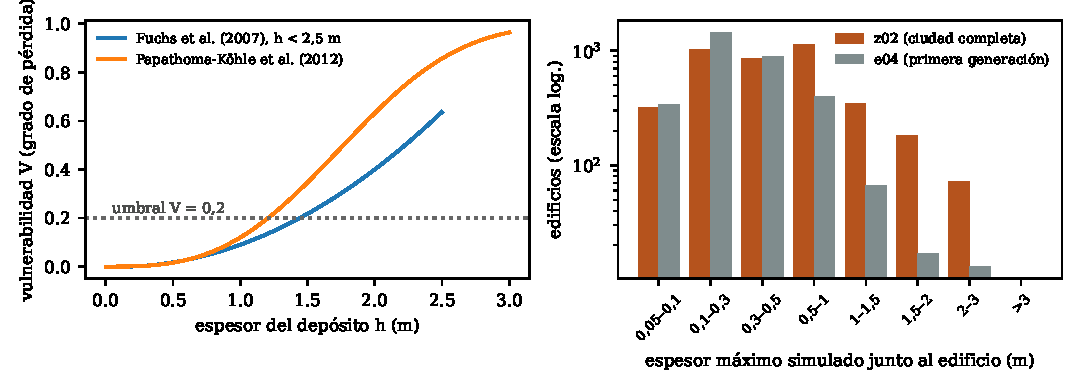
\includegraphics[width=\textwidth]{vulnerabilidad}
\caption{Izquierda: curvas de vulnerabilidad de \citet{fuchs2007} (solo en su dominio) y \citet{papathoma2012}. Derecha: espesor máximo simulado junto a los edificios expuestos, en la hipótesis seleccionada con la ciudad completa (z02) y en la primera generación (e04), en escala logarítmica.}\label{fig:vulnerabilidad}
\end{figure}

\begin{table}[htbp]\centering\small
\caption{Pérdida relativa esperada con el espesor máximo simulado junto a cada edificio como intensidad. $\Sigma V$: pérdida relativa agregada (no es un conteo de edificios destruidos). Fuchs solo en su dominio ($h<\SI{2,5}{m}$); los edificios con $h\geq\SI{2,5}{m}$ se informan aparte. Viviendas: asignadas a los edificios con $V\geq0{,}2$.}\label{tab:danio}
\begin{adjustbox}{max width=\textwidth}\begin{tabular}{p{.34\textwidth}rrrrrrr}\toprule
Escenario & \multicolumn{3}{c}{Fuchs et al. (2007)} & \multicolumn{3}{c}{Papathoma-Köhle et al. (2012)} & $h\geq\SI{2,5}{m}$\\\cmidrule(lr){2-4}\cmidrule(lr){5-7}
 & $\Sigma V$ & Edif. $V\geq0{,}2$ & Viv. & $\Sigma V$ & Edif. $V\geq0{,}2$ & Viv. & Edif.\\\midrule
Seleccionada: cauce + brazos sur + lluvia (300 mil m³) & 187,1 & 271 & 366 & 275,8 & 425 & 593 & 15\\
Ídem con más rugosidad fuera de calles & 174,9 & 244 & 346 & 256,9 & 398 & 594 & 12\\
Solo cauce principal (300 mil m³) & 163,9 & 264 & 305 & 248,4 & 390 & 498 & 16\\
Solo cauce principal (150 mil m³) & 83,3 & 131 & 117 & 123,3 & 203 & 199 & 4\\
Hipotético: colector 30 m³/s & 121,3 & 169 & 151 & 181,2 & 264 & 246 & 12\\
Hipotético: colector 100 m³/s & 107,6 & 162 & 129 & 162,8 & 242 & 192 & 12\\
Primera generación (modelo con 1.103 edificios; exposición sobre 42.018 huellas) & 43,4 & 34 & 26 & 55,4 & 52 & 38 & 1\\
\bottomrule\end{tabular}\end{adjustbox}\end{table}

\paragraph{Pérdida esperada.} Con la ciudad completa, los espesores junto a los edificios son mucho mayores que en la primera generación: 599 edificios tienen más de \SI{1}{m}, frente a 96 antes (figura~\ref{fig:vulnerabilidad}). En la hipótesis seleccionada:
\begin{itemize}
\item la pérdida relativa agregada es 187 con la curva de Fuchs y 276 con la de Papathoma-Köhle;
\item entre 271 y 425 edificios tienen $V\geq0{,}2$, con 366 a 593 viviendas asignadas;
\item 15 edificios quedan fuera del dominio de Fuchs (cuadro~\ref{tab:danio}).
\end{itemize}

\begin{figure}[htbp]\centering
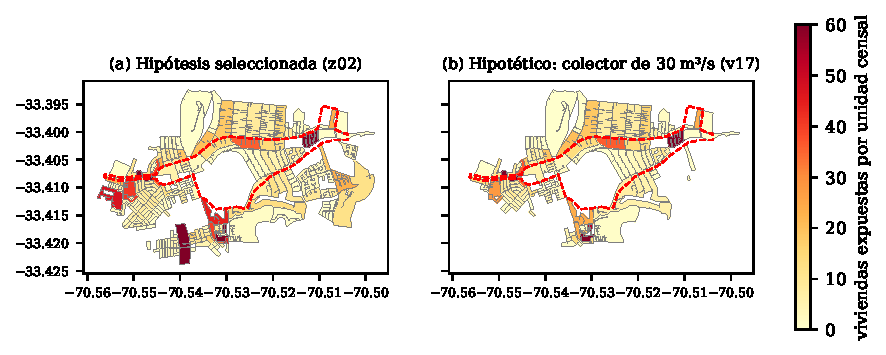
\includegraphics[width=\textwidth]{manzanas}
\caption{Viviendas expuestas por unidad censal (Censo 2017, ponderación areal) con más de \SI{5}{cm} de barro simulado, y zona afectada oficial \citep{bbnn2026visor} en línea roja discontinua. (a) Hipótesis seleccionada. (b) Escenario hipotético con la capacidad del colector de Bulnes Correa fijada en \SI{30}{m^3/s}.}\label{fig:manzanas}
\end{figure}

\paragraph{Comparación descriptiva con las cifras oficiales.}
\begin{table}[htbp]\centering\small
\caption{Comparación descriptiva con los balances oficiales (hipótesis seleccionada, z02). Las categorías calculadas y administrativas no son equivalentes.}\label{tab:contraste}
\begin{tabular}{p{.22\textwidth}p{.34\textwidth}p{.34\textwidth}}\toprule
Indicador & Cifra oficial & Este estudio (calculado)\\\midrule
Viviendas afectadas & Senapred, balance preliminar: 2.361 (75 con daño mayor y 2.286 con daño menor); balance posterior: 56 destruidas, 40 con daño mayor y 1.960 con daño menor; municipio: 1.960--2.015 & 2.221 (A) y 5.827 (B) a más de \SI{5}{cm}; sensibilidad: 1.900--6.551\\
Daño severo & Senapred: 75 con daño mayor (preliminar); 56 destruidas y 40 con daño mayor (posterior); municipio: 55 inhabitables & 366--593 viviendas en edificios con $V\geq0{,}2$; 271--425 edificios con $V\geq0{,}2$\\
Predios afectados & Visor de emergencia: 2.266 predios afectados (91~\% dentro de la zona afectada) & El estudio principal moja 717 de ellos (32~\%)\\
Calles & Municipio: \SI{15}{km} de avenidas dañadas & \SI{19,5}{km} de calles con barro, \SI{16,5}{km} de vías principales a terciarias\\
Personas & Senapred: 384 damnificados y más de 1.200 rescatados (posterior) & 7.052--17.883 personas censales asignadas al área (concepto distinto: exposición)\\
\bottomrule\end{tabular}\end{table}
\noindent Sobre la pregunta P1, la ponderación areal queda en el orden de las viviendas afectadas informadas, y la asignación dasimétrica más de dos veces por encima. Ninguno de los dos métodos está validado para elegir entre ellos. Sobre la pregunta P2, las viviendas con pérdida esperada significativa superan varias veces a las informadas con daño mayor o destruidas.

\section{Discusión}
\paragraph{Por qué la pérdida esperada sale alta.} Las curvas se aplican al espesor máximo del flujo en la calle contigua, no al depósito junto a cada vivienda. Con los edificios representados como bloques impermeables, el barro no entra a los lotes y se concentra en las calles con 1 a \SI{2}{m}; en la realidad, parte del barro entró a antejardines y primeros pisos, y otra parte se detuvo en rejas y muros. Además, las curvas provienen de eventos alpinos con velocidades y tipologías distintas, y no consideran la velocidad ni la presión. Por eso las cifras de daño sirven como cota superior condicionada al modelo, no como estimación del daño ocurrido.
\paragraph{La propagación hereda un error espacial.} En el estudio principal, la prueba con observaciones reservadas resultó desfavorable: la hipótesis seleccionada deja barro junto a 19 de 49 equipamientos afectados oficiales. El modelo moja cerca del 20~\% del área de la zona oficial y el 32~\% de sus predios afectados, y se extiende fuera de ella. La exposición calculada combina, por lo tanto, viviendas fuera de la zona oficial que el modelo moja y viviendas dentro de ella que no moja. Que la ponderación areal quede cerca del total oficial no significa que identifique las mismas viviendas.
\paragraph{Qué cambió respecto de la versión anterior.} La primera generación del modelo, con 1.103 edificios, repartía el barro en láminas delgadas sobre un área amplia. Por eso sus cifras de exposición quedaban, por coincidencia de órdenes de magnitud, cerca de los balances. La ciudad completa encauza el flujo, profundiza las calles y separa los dos métodos de asignación. La concordancia descriptiva de la versión anterior no se mantiene y no debe citarse como evidencia.
\paragraph{Supuestos y sesgos.}
\begin{itemize}
\item El Censo 2017 no refleja el crecimiento posterior.
\item Las huellas detectadas automáticamente pueden fusionar o dividir edificios, y la asignación dasimétrica no distingue usos residenciales de no residenciales.
\item Las 18 unidades sin huellas elegibles se asignan por área.
\item No se estima el daño a contenidos, vehículos ni infraestructura pública.
\end{itemize}

\section{Conclusiones}
\begin{enumerate}
\item Con la ciudad completa y la hipótesis seleccionada, entre 1.900 y 6.551 viviendas censales se asignan al área con barro simulado, según el método y los supuestos. El método de asignación es la mayor fuente de variación.
\item La pérdida esperada calculada con curvas de vulnerabilidad supera varias veces las viviendas informadas con daño mayor o destruidas. Se atribuye principalmente a usar el espesor del flujo en la calle como intensidad y a representar los edificios como bloques. Debe leerse como una cota superior condicionada al modelo.
\item La propagación no reproduce la distribución espacial de la afectación oficial (prueba reservada desfavorable). Por eso estas cifras no identifican viviendas afectadas ni sirven para asignar ayudas.
\item El método es reproducible con datos públicos. Los siguientes pasos son una intensidad junto a la vivienda (depósito o entrada al lote), una representación de edificios que admita la entrada del barro y un contraste con un inventario independiente de daño por vivienda.
\end{enumerate}

\section*{Disponibilidad de datos y código}
Los programas y los resultados agregados están en la página de datos del estudio (\url{https://aluvion.hirely.cl/datos.html}):
\begin{itemize}
\item \texttt{exposicion3.py} y \texttt{figura\_exposicion3.py};
\item \texttt{res/exposicion3\_20261011.json}.
\end{itemize}
Solo se publican agregados. La versión anterior, basada en la primera generación, se conserva en \url{https://aluvion.hirely.cl/paper/versiones/}.

\bibliographystyle{apacite}
\bibliography{referencias}
\end{document}
